\documentclass[a4paper, titlepage]{article}
\usepackage[round, sort, numbers]{natbib}
\usepackage[utf8]{inputenc}
\usepackage{amsfonts, amsmath, amssymb, amsthm}
\usepackage{color}
\usepackage{listings}
\usepackage{mathtools}
\usepackage{paralist}
\usepackage{parskip}
\usepackage{subfig}
\usepackage{tikz}
\usepackage{titlesec}

\numberwithin{figure}{section}
\numberwithin{table}{section}

\usetikzlibrary{arrows, automata, backgrounds, petri, positioning}
\tikzstyle{place}=[circle, draw=blue!50, fill=blue!20, thick]
\tikzstyle{transition}=[rectangle, draw=black!50, fill=black!20, thick]

% define new commands for sets and tuple
\newcommand{\setof}[1]{\ensuremath{\left \{ #1 \right \}}}
\newcommand{\tuple}[1]{\ensuremath{\left \langle #1 \right \rangle }}
\newcommand{\card}[1]{\ensuremath{\left \vert #1 \right \vert }}

\makeatletter
\newcommand\objective[1]{\def\@objective{#1}}
\newcommand{\makecustomtitle}{%
	\begin{center}
		\huge\@title \\
		[1ex]\small Dimitri Racordon \\ \@date
	\end{center}
	\@objective
}
\makeatother

\begin{document}

  \title{Outils formels de Modélisation \\ 2\textsuperscript{ème} séance d'exercices}
  \author{Dimitri Racordon}
  \date{29.09.17}
	\objective{
		Dans cette séance d'exercices, nous allons manipuler quelques définitions formelles
		relatives aux réseaux de Petri et étudier leur signification avec des exemples.
	}

	\makecustomtitle

  \section{Syntaxe et sémantique ($\bigstar$)}
		Répondez aux questions suivantes:
		\begin{enumerate}
			\item Quelle est la différence entre les notions de syntaxe et de sémantique?
			\item Ecrivez la syntaxe d'un automate à états finis $\mathcal{A}$ sur un alphabet $\Sigma$.
			\item Soit $\mathcal{A}$ un automate à états finis non déterministe.
            Décrivez la sémantique d'un opérateur $\rightarrow$ qui dénote la lecture
            d'un caractère $c\in\Sigma$ par l'automate $\mathcal{A}$.
		\end{enumerate}

  \section{Et maintenant on code! ($\bigstar\bigstar\bigstar$)}
    Ecrivez une structure de données permettant de représenter un automate à états finis
    $\mathcal{A}$ sur un alphabet $\Sigma$, puis écrivez une fonction (ou méthode)
    permettant de simuler la lecture d'un caractère.

  \section{Définition formelle des réseaux de Petri ($\bigstar\bigstar$)}
		Répondez aux questions suivantes:
		\begin{enumerate}
			\item De manière informelle, qu'est-ce que le marquage d'un réseau de Petri? Que dénote-t-il?
			\item Ecrivez la syntaxe d'un réseau de Petri.
			\item Ecrivez la sémantique d'un réseau de Petri.
		\end{enumerate}

  \section{Simulations ($\bigstar\bigstar$)}
    A l'aide de l'outil PetriKit (https://github.com/kyouko-taiga/PetriKit),
    représentez le réseau de Petri de la figure \ref{fig:bezout},
    puis répondez aux questions suivantes:

    \begin{enumerate}
			\item La transition $t_2$ est-elle tirable?
			\item Donnez un marquage possible du réseau après 100 tirs de transitions.
		\end{enumerate}

    \begin{figure}[ht]
      \centering
        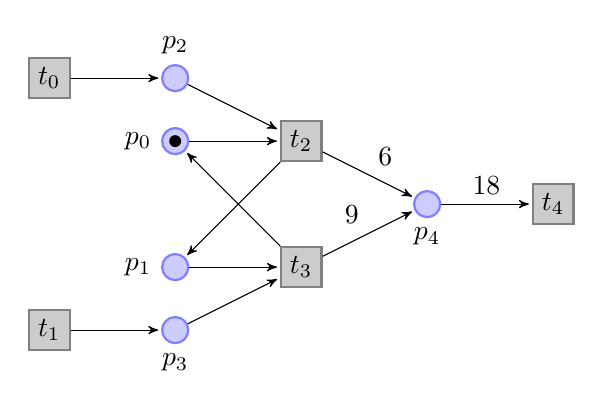
\begin{tikzpicture}[node distance=16mm, >=stealth', bend angle=45, auto]
          \node[place] (p4) [label=below:$p_4$] {};
          \node[place,tokens=1] (p0) [left of=p4,xshift=-16mm,yshift=8mm,label=left:$p_0$] {};
          \node[place] (p1) [left of=p4,xshift=-16mm,yshift=-8mm,label=left:$p_1$] {};
          \node[place] (p2) [above of=p0,yshift=-8mm,label=above:$p_2$] {};
          \node[place] (p3) [below of=p1,yshift=8mm,label=below:$p_3$] {};

          \node [transition] (t0) [left of=p2] {$t_0$}
                edge [post] (p2);
          \node [transition] (t1) [left of=p3] {$t_1$}
                edge [post] (p3);
          \node [transition] (t2) [right of=p0] {$t_2$}
                edge [pre] (p0)
                edge [pre] (p2)
                edge [post] node {6} (p4)
                edge [post] (p1);
          \node [transition] (t3) [right of=p1] {$t_3$}
                edge [pre] (p1)
                edge [pre] (p3)
                edge [post] node {9} (p4)
                edge [post] (p0);
          \node [transition] (t4) [right of=p4] {$t_4$}
                edge [pre] node[swap] {18} (p4);
        \end{tikzpicture}
      \caption{Réseau exposant des propriétés algébriques intéressantes}
      \label{fig:bezout}
    \end{figure}

  \section{Complémentaire mon cher ($\bigstar\bigstar$)}
		En cours, nous avons vu qu'il pouvait parfois être désirable d'ajouter une place
    qui limite le nombre de tokens pouvant être produits dans une autre place.
    On appelle généralement ces ajouts des \emph{places complémentaires}.

		Pour chacun des réseaux de Petri de la figure \ref{fig:unbound},
    ajoutez des places complémentaires pour limiter le nombre de jetons à 3
    dans chaque place \emph{sans autrement modifier le comportement du réseau}.

    \begin{figure}[ht]
      \centering
			\begin{tabular}{c}
      \subfloat[]{%
        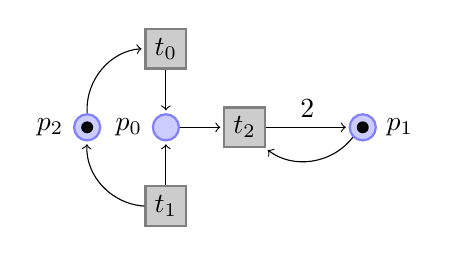
\begin{tikzpicture}[bend angle=45]
          \node[place] (p0) [label=left:$p_0$] {};
					\node[place,tokens=1] (p1) [right of=p0, xshift=1.5cm, label=right:$p_1$] {};
					\node[place,tokens=1] (p2) [left of=p0, label=left:$p_2$] {};
          \node [transition] (t0) [above of=p0] {$t_0$}
								edge [pre, bend right] (p2)
                edge [post] (p0);
          \node [transition] (t1) [below of=p0] {$t_1$}
                edge [post] (p0) edge [post, bend left] (p2);
          \node [transition] (t2) [right of=p0] {$t_2$}
							  edge [pre] (p0) edge [pre, bend right] (p1)
                edge [post] node[above] {2} (p1);
        \end{tikzpicture}
      } \\
      \subfloat[]{%
        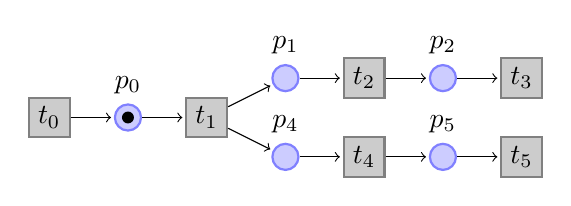
\begin{tikzpicture}
          \node[place,tokens=1] (p0) [label=above:$p_0$] {};
					\node[place] (p1) [right of=p0, xshift=1cm, yshift=0.5cm, label=above:$p_1$] {};
					\node[place] (p2) [right of=p1, xshift=1cm, label=above:$p_2$] {};

					\node[place] (p4) [right of=p0, xshift=1cm, yshift=-0.5cm, label=above:$p_4$] {};
					\node[place] (p5) [right of=p4, xshift=1cm, label=above:$p_5$] {};

          \node [transition] (t0) [left of=p0] {$t_0$}
							  edge [post] (p0);
          \node [transition] (t1) [right of=p0] {$t_1$}
							  edge [pre] (p0)
                edge [post] (p1)
								edge [post] (p4);
          \node [transition] (t2) [right of=p1] {$t_2$}
							  edge [pre] (p1) edge [post] (p2);
          \node [transition] (t3) [right of=p2] {$t_3$}
							  edge [pre] (p2);
          \node [transition] (t4) [right of=p4] {$t_4$}
							  edge [pre] (p4) edge [post] (p5);
          \node [transition] (t5) [right of=p5] {$t_5$}
							  edge [pre] (p5);
        \end{tikzpicture}
      }
			\end{tabular}
			\caption{Réseaux de Petri non-bornés}
			\label{fig:unbound}
    \end{figure}

		Ecrivez ensuite la définition formelle d'une place complémentaire.
    Votre définition doit être de la forme suivantes:
    \emph{Soit $N$ un réseau de Petri tel que ... $p'\in P$ est dite complémentaire à $p \in P$ si et seulement si ...}

\end{document}
